% -*- TeX-master: "User_guide"; fill-column: 75 -*-

\section[Writing your first JSBML application]{\emph{Hello World}: writing your first JSBML applications}
\label{sec:hello-world}

In this section, we present two examples of using JSBML. The first is a
program that reads a file containing an SBML document and displays its
components in a Java \JTree graphical object. The second example
illustrates the creation of an object representing an SBML document (which,
in JSBML, is represented programmatically using an object of class
\SBMLDocument), as well as writing that object to a file. These basic
examples should help serve as a foundation for writing your own, more
elaborate programs.


\subsection{Reading and visualizing an \codeNC{SBMLDocument} object}

\fig{fig:JSBMLvisualizer-source} shows the listing of a very simple
program called ``\code{JSBMLvisualizer}''. When it is run, it expects to
be given the path name of a valid SBML file as \index{SBML!XML file} its
sole argument. The program uses the static method \code{read()} defined
by the JSBML object class \SBMLReader to read the file; \SBMLReader
returns an object of class \SBMLDocument, the main SBML document
container in JSBML.  Next, the program constructs a new
\code{JSBMLvisualizer} object, which is derived from the standard Java
\JFrame class. It invokes the class constructor (line 9) with the
identifier of the model in the SBML file, obtained by calling
\code{getModel().getId()} on the \SBMLDocument object; this sets the
\JFrame's title to the identifier of the model. Since JSBML's \SBase
object (and all objects derived from it) implement the \TreeNode
interface, it is possible to create a \JTree directly from the
information in an \SBMLDocument object instance.  (To keep our examples
short and focused on the essentials of using JSBML, we have omitted
error checking steps.  A real application program should guard against
various situations, such as \code{getModel()} or \code{getId()} returning \code{null}, and
take steps to deal with them appropriately. You might also like to read SBML files 
in a separate thread and monitor the progress of reading the file in some progress bar.)

To compile and execute ``\code{JSBMLvisualizer}'', you would need to do
the following sequence of commands:

\newcommand{\classpath}{\code{\emph{\color{winered}classpath}}\xspace}

\begin{example}[style=bash, title={Compiling and executing the example program.}]
  javac -classpath |\classpath|JSBMLvisualizer.java
  java -classpath |\classpath|JSBMLvisualizer
\end{example}

In the example commands above, replace the placeholder text \classpath with
the actual Java class path for the JSBML libraries and its dependencies on
your particular computer; we do not show an exact value here because it
depends on where you have installed the JAR files for JSBML and the
third-party libraries.

\begin{figure}[ht]
  \exampleFile{src/JSBMLvisualizer.java}
  \caption{Parsing and visualizing the content of an SBML file.}
  \label{fig:JSBMLvisualizer-source}
  \index{graphical user interface!\code{JFrame}}
\end{figure}

\begin{wrapfigure}[27]{r}{2.55in}
  \centering
  \vspace*{-1em}
  \setlength{\captionmargin}{1.8em}
  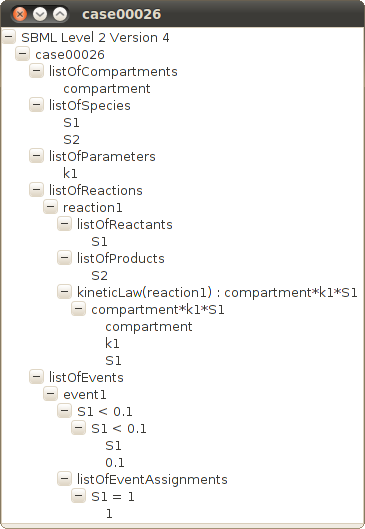
\includegraphics[width=.32\textwidth]{%
    ../posters/2010_ICSB_and_COMBINE/JSBMLvisualizerTransparent.png}
  \caption[Tree representation of an SBML file]{Tree representation of
    the contents of the SBML test file ``\code{case00026}.xml''. In JSBML,
    the hierarchically structured \SBMLDocument can be traversed
    recursively because all instances of \SBase, the parent class,
    implement the interface \TreeNode.}
  \label{fig:JSBMLvisualizer-output}
\end{wrapfigure}
\fig{fig:JSBMLvisualizer-output} shows the example output when
applying the program to an SBML test model. \index{SBML!test cases} Each
element in the model shows up as an item in the hierarchy displayed by the
Java \JTree object. In the working application, the user can click on the
control boxes (i.e., the boxed ``+'' and ``-'' symbols next to the element
names) to collapse or expand the views of the substructures of an SBML
model.

We hasten to add that this simple program lacks many features that a proper
application should possess.  We kept this example purposefully as simple as
possible so that it is easier to focus on the main point of the example
(which is, how read to an SBML file).  Perhaps the most important missing
aspect is checking for and handling errors that may be encountered when
trying to read and parse the file given as argument to the program.  Not
all SBML files are valid, owing to the unfortunate reality that \emph{not
  all software tools in the world produce syntactically and semantically
  correct SBML}. The JSBML library is flexible and attempts to carry on in
the face of problems, because it is the responsibility of the calling
application to decide when and how problems should be handled. A realistic
application should be coded defensively: it should be prepared for the
possibility of receiving badly-formed input, check for any warnings and
errors reported by \SBMLReader when it attempts to read the SBML file, and
deal with them appropriately. Elsewhere in this document, we provide
examples of checking for errors.

Reading a file is nice, but what about writing an SBML file?  That is the
topic of the next example.

% FIXME tell people where to find the source code to the examples.


\subsection{Creating and writing an \codeNC{SBMLDocument} object}

Our next example, shown in \fig{fig:JSBMLexample-source},
illustrates how to construct an in-memory representation of an SBML model
and write it to a file. The program first creates an \SBMLDocument object,
then attaches a \Model object to it, and then to the \Model adds one
\Compartment, two \Species, and one \Reaction objects. To write the
contents to a file named ``\code{test.xml}'', the program uses a static
method on the JSBML class \SBMLWriter. 

This program also illustrates the preferred approach to the creation of JSBML object instances. 
The only constructor you should need to use is the constructor of the \SBMLDocument, specifying
the SBML Level and Version you want to use. Each JSBML class should have  
\code{create\emph{XYZ}} methods, where \code{\emph{XYZ}} is the subclass name. 
For example, you may have \code{model.createSpecies(String)}, \code{model.createReaction(String)}
or \code{reaction.createReactant()}. These methods will guarantee that callers create a proper
representation of the SBML model.  

\begin{figure}[bht]
  \vspace*{-1ex}
  \exampleFile{src/JSBMLexample.java}
  \vspace*{-1.5ex}
  \caption{Creating a new \code{SBMLDocument} object and writing its content
    into a file.}
  \label{fig:JSBMLexample-source}
\end{figure}


\section{More examples}

\fig{lst:LibSBMLio} illustrates the conversion of libSBML data structures
into JSBML data objects. \fig{lst:PluginAction} demonstrates the
implementation of CellDesigner's abstract class \code{PluginAction} and
\fig{lst:Plugin1} gives a complete example for writing CellDesigner plugins
with JSBML.  \index{CellDesigner} More detailed explanations of JSBML's
modules can be found in \sec{sec:jsbml-modules-details}, and more complex
examples of using JSBML are available from the JSBML SourceForge repository.
(Please see \sec{sec:jsbml-repo-examples} for information about how to obtain
them.)
